% --- Program Section ---

\newprogram{Program 15}{ Build a GraphBacktracker class featuring graph-coloring(m: int) -> List[int] and
hamiltonian-cycle() -> List[int] methods returning vertex-color mappings and valid path
cycles.}
\subsection*{Code}


\begin{lstlisting}[language=python]
from typing import List


class GraphBacktracker:

    def __init__(self, graph: List[List[int]]):
        self.graph = graph
        self.n = len(graph)

    # --------------------------------
    # Graph Coloring
    # --------------------------------
    def graph_coloring(self, m: int) -> List[int]:
        colors = [0] * self.n

        def is_safe(vertex, color):
            for neighbor in range(self.n):
                if self.graph[vertex][neighbor] and colors[neighbor] == color:
                    return False
            return True

        def backtrack(vertex):
            if vertex == self.n:
                return True

            for color in range(1, m + 1):
                if is_safe(vertex, color):
                    colors[vertex] = color

                    if backtrack(vertex + 1):
                        return True

                    colors[vertex] = 0

            return False

        if backtrack(0):
            return colors

        return []


    # --------------------------------
    # Hamiltonian Cycle
    # --------------------------------
    def hamiltonian_cycle(self) -> List[int]:
        if self.n == 0:
            return []

        path = [-1] * self.n
        path[0] = 0

        def is_safe(vertex, position):
            # Must be connected to previous vertex
            if not self.graph[path[position - 1]][vertex]:
                return False

            # Vertex must not already be in path
            if vertex in path:
                return False

            return True

        def backtrack(position):
            if position == self.n:
                # Last vertex must connect to first vertex
                return self.graph[path[-1]][path[0]] != 0

            for vertex in range(1, self.n):
                if is_safe(vertex, position):
                    path[position] = vertex

                    if backtrack(position + 1):
                        return True

                    path[position] = -1

            return False

        if backtrack(1):
            # Add starting vertex to show complete cycle
            return path + [path[0]]

        return []


# --------------------------------
# Example Graph
# --------------------------------

graph = [
    [0, 1, 1, 1],
    [1, 0, 1, 1],
    [1, 1, 0, 1],
    [1, 1, 1, 0]
]

solver = GraphBacktracker(graph)


# Graph Coloring
print("Graph Coloring:")
print(solver.graph_coloring(3))


# Hamiltonian Cycle
print("\nHamiltonian Cycle:")
print(solver.hamiltonian_cycle())
\end{lstlisting}

\subsection*{Output}
\begin{center}
    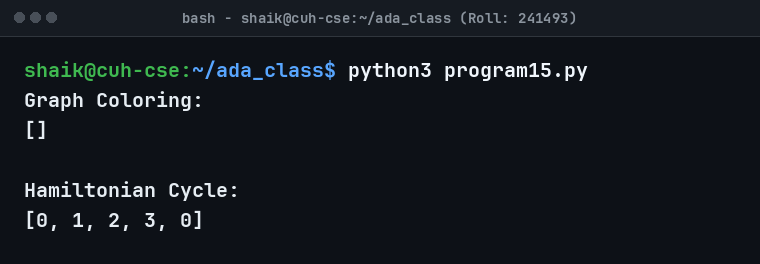
\includegraphics[width=0.88\textwidth]{Images/output_screenshot15.png}
\end{center}

\subsection*{GitHub Scan Code}
\begin{center}
    \begin{minipage}{0.3\textwidth}
        \centering
        % Generates a 2.5cm high QR code directly linking to the code file
        \qrcode[height=3.5cm]{https://github.com/gytdrop/ada_class/blob/main/program15.py} \\[0.2cm]
        \scriptsize\ttfamily Scan to view source code 
    \end{minipage}
\end{center}


% Add a horizontal line that indicates the END of the program.
\vspace{1cm}
\begin{center}
    \rule{1\textwidth}{1pt} % Clean, centered 1pt thick horizontal line
\end{center}